%%%%%%%%%%%%%%%%%%%%%%%%%%%%%%%%%%%%%%%%%%%%%%%%%%%%%%%%%%%%%%%%%%%%%%%%%%%
% Chapter: Programming
% Examples: examples/programming (assembly on the Pico in C and Rust, a
% host-tested Rust library, MicroPython, Python, C register access)
%%%%%%%%%%%%%%%%%%%%%%%%%%%%%%%%%%%%%%%%%%%%%%%%%%%%%%%%%%%%%%%%%%%%%%%%%%%

%%%%%%%%%%%%%%%%%%%%%%%%%%%%%%%%%%%%%%%%%%%%%%%%%%%%%%%%%%%%%%%%%%%%%%%%%%%
\section{From Source Code to Firmware}
%%%%%%%%%%%%%%%%%%%%%%%%%%%%%%%%%%%%%%%%%%%%%%%%%%%%%%%%%%%%%%%%%%%%%%%%%%%
\nsl{Embedded software is developed on a PC and runs on a different
processor: it is cross-compiled. The toolchain translates the source code
into machine code for the target, the linker places code and data at the
addresses of the target's memory, and a programming tool writes the result
into the flash. This chapter starts with these steps. Then it looks at the
languages used in this lecture, from assembly through C and Rust to
MicroPython, and ends with systematic debugging. Several examples run on the
Raspberry Pi Pico in Wokwi again.
\newpage}

\begin{description}
\item[{\rot\bf The build process}]~\\[-3ex]
\begin{figure}[!hbtp]
\begin{center}
\resizebox{0.95\textwidth}{!}{%
\begin{tikzpicture}[font=\sffamily\small,>=Stealth,
	b/.style={draw,thick,rounded corners,minimum height=10mm,text width=20mm,align=center}]
	\node[b,fill=gray!10] (src) at (0,0) {source\\.c .rs .S};
	\node[b,fill=blue!10] (cc) at (3,0) {compiler /\\assembler};
	\node[b,fill=gray!10] (obj) at (6,0) {object files\\.o};
	\node[b,fill=blue!10] (ld) at (9,0) {linker};
	\node[b,fill=gray!10] (elf) at (12,0) {ELF file};
	\node[b,fill=green!10] (img) at (15,0) {.bin / .hex\\/ .uf2};
	\node[b,fill=orange!15] (lds) at (9,-2) {linker script\\memory map};
	\node[b,fill=orange!15] (lib) at (6,-2) {libraries,\\start-up code};
	\draw[->,thick] (src) -- (cc); \draw[->,thick] (cc) -- (obj); \draw[->,thick] (obj) -- (ld);
	\draw[->,thick] (ld) -- (elf); \draw[->,thick] (elf) -- node[above,font=\sffamily\scriptsize]{objcopy} (img);
	\draw[->,thick] (lds) -- (ld); \draw[->,thick] (lib) -- (ld);
\end{tikzpicture}}
\caption{From source code to the image in the flash}
\end{center}
\end{figure}
\bi
	\ite \textbf{cross compiler}, named after the target: \texttt{arm-none-eabi-gcc} (ARM, no OS), \texttt{riscv32-esp-elf-gcc}; in Rust a target triple such as \texttt{thumbv6m-none-eabi}
	\ite the \textbf{linker} combines all object files and assigns addresses according to the linker script (\texttt{memory.x} in our Rust examples: flash at 0x1000\,0000, RAM at 0x2000\,0000)
	\ite the \textbf{ELF} file contains code, data, symbols and debug information -- the debugger needs it; the flash only needs the raw image
\ei
\os{\newpage}

\item[{\rot\bf Sections and start-up}]~\\[-3ex]
\bi
	\ite \texttt{.text}: machine code (flash); \texttt{.rodata}: constants (flash)
	\ite \texttt{.data}: initialised variables -- the initial values are in flash, the variables in RAM
	\ite \texttt{.bss}: variables initialised with zero (RAM only)
	\ite the \textbf{start-up code} runs before \texttt{main}: set the stack pointer (from the vector table), copy \texttt{.data} from flash to RAM, fill \texttt{.bss} with zeros, set up clocks, then call \texttt{main}
	\ite in Rust \texttt{cortex-m-rt} provides this code and the attribute \texttt{\#[entry]}
\ei
\begin{lstlisting}[language={}]
$ llvm-size -A target/thumbv6m-none-eabi/release/gpio_blink   # addresses in hex
section        size        addr
.vector_table   192   0x10000100
.boot2          256   0x10000000      <- 2nd stage bootloader of the RP2040
.text          2940   0x100001c0
.rodata         360   0x10000b3c
.bss              4   0x20000000
\end{lstlisting}
\bi
	\ite the same blink program with the Arduino core: about 314\,KB code -- the core always links USB, serial and file system support
\ei
\os{\newpage}

\item[{\rot\bf Getting the program onto the chip}]~\\[-3ex]
\bi
	\ite \textbf{bootloader in ROM} or flash: receives the image over USB or UART
	\bi
		\ite RP2040: hold BOOTSEL, the Pico appears as a USB drive -- copy a \texttt{.uf2} file onto it
		\ite ESP32: ROM bootloader via the serial port (\texttt{esptool}, \texttt{espflash})
	\ei
	\ite \textbf{debug probe} via SWD or JTAG (see section Debugging): programming and debugging with the same cable
	\ite in production: programming on the panel, in-circuit test, unique keys and serial numbers per device
	\ite \textbf{over the air} updates: the running firmware downloads a new image into a second flash partition and switches after a check -- needs a bootloader that can roll back
\ei
\os{\newpage}
\end{description}

%%%%%%%%%%%%%%%%%%%%%%%%%%%%%%%%%%%%%%%%%%%%%%%%%%%%%%%%%%%%%%%%%%%%%%%%%%%
\section{Programming in Assembly}
%%%%%%%%%%%%%%%%%%%%%%%%%%%%%%%%%%%%%%%%%%%%%%%%%%%%%%%%%%%%%%%%%%%%%%%%%%%
\nsl{Today almost nobody writes complete programs in assembly. Compilers
generate good code, and C and Rust are portable and much easier to maintain.
Still, every embedded developer must be able to read assembly. You need it
to understand what the compiler made of your code, to analyse a crash in
the debugger, and to write the few parts that cannot be expressed in a high
level language, such as start-up code, context switches and special
instructions. We use the Cortex-M0+ of the RP2040 as our example. Its
instruction set (Thumb, ARMv6-M) is small enough to be learned in a few
hours.}

\begin{description}
\item[{\rot\bf Registers of the Cortex-M0+}]~\\[-3ex]
\bi
	\ite 16 registers of 32 bit
	\bi
		\ite \texttt{r0}--\texttt{r12}: general purpose (most 16 bit instructions can only use \texttt{r0}--\texttt{r7})
		\ite \texttt{r13} = \texttt{sp}: stack pointer (two of them: main and process stack)
		\ite \texttt{r14} = \texttt{lr}: link register, return address of a function call
		\ite \texttt{r15} = \texttt{pc}: program counter
	\ei
	\ite \textbf{xPSR} status register with the flags of the last arithmetic instruction
	\bi
		\ite \textbf{N} negative, \textbf{Z} zero, \textbf{C} carry (unsigned overflow), \textbf{V} overflow (signed)
		\ite only instructions with an \texttt{s} suffix (\texttt{adds}, \texttt{subs}) and comparisons (\texttt{cmp}) set the flags
	\ei
	\ite all data processing works on registers -- memory only via \texttt{ldr}/\texttt{str} (load/store architecture)
\ei
\os{\newpage}

\item[{\rot\bf Instructions (selection)}]~\\[-3ex]
\begin{center}
\resizebox{\textwidth}{!}{%
\begin{tabular}{|l|l|l|}
\hline
\textbf{group} & \textbf{examples} & \textbf{meaning} \\
\hline
move & \texttt{movs r0, \#5} \quad \texttt{mov r1, r2} & r0 = 5 (8 bit immediate), r1 = r2 \\
arithmetic & \texttt{adds r0, r1, r2} \quad \texttt{subs r1, r1, \#1} \quad \texttt{muls r0, r1} & r0 = r1 + r2, r1 = r1 - 1, r0 = r0 $\cdot$ r1 \\
logic, shift & \texttt{ands r0, r1} \quad \texttt{orrs} \quad \texttt{eors} \quad \texttt{lsls r0, r0, \#2} & bitwise AND, OR, XOR; shift left \\
compare & \texttt{cmp r1, \#0} \quad \texttt{cmp r3, r1} & compute r1 - 0, set flags only \\
load & \texttt{ldr r0, [r1]} \quad \texttt{ldrh r3, [r0, \#2]} \quad \texttt{ldrb r2, [r0, r1]} & 32 / 16 / 8 bit from memory \\
store & \texttt{str r0, [r1, \#4]} \quad \texttt{strh} \quad \texttt{strb} & 32 / 16 / 8 bit to memory \\
constant & \texttt{ldr r0, =0xd000001c} & 32 bit constant from a literal pool in flash \\
stack & \texttt{push \{r4, lr\}} \quad \texttt{pop \{r4, pc\}} & save registers / restore and return \\
branch & \texttt{b label} \quad \texttt{beq} \quad \texttt{bne} \quad \texttt{blt} \quad \texttt{bhs} & jump, conditional on the flags \\
call, return & \texttt{bl function} \quad \texttt{bx lr} & call (return address in lr), return \\
\hline
\end{tabular}}
\end{center}
\bi
	\ite conditions: \texttt{eq}/\texttt{ne} (Z), signed \texttt{lt}/\texttt{ge}/\texttt{gt}/\texttt{le}, unsigned \texttt{lo}/\texttt{hs}/\texttt{hi}/\texttt{ls}
\ei
\os{\newpage}

\item[{\rot\bf Calling convention (AAPCS)}]~\\[-3ex]
\bi
	\ite the rules that let C, Rust and assembly functions call each other
	\ite arguments in \texttt{r0}--\texttt{r3}, further arguments on the stack
	\ite return value in \texttt{r0} (64 bit values in \texttt{r0}+\texttt{r1})
	\ite \texttt{r0}--\texttt{r3} and \texttt{r12} may be changed by the called function (caller-saved)
	\ite \texttt{r4}--\texttt{r11} must have the same value after the call (callee-saved) -- save them with \texttt{push} if you use them
	\ite the stack grows downwards and is 8 byte aligned at function calls
	\ite the RISC-V equivalent: arguments in \texttt{a0}--\texttt{a7}, return value in \texttt{a0}, callee-saved \texttt{s0}--\texttt{s11}, return address in \texttt{ra}
\ei
\os{\newpage}

\item[{\rot\bf Our own assembly function}]~\\[-3ex]
\begin{lstlisting}[language={}]
@ uint32_t asm_sum(const uint16_t *a, int n)    file sum_m0.S
@ AAPCS: a in r0, n in r1, result in r0. Only r0..r3 are used.
    .syntax unified
    .cpu cortex-m0plus
    .thumb
    .global asm_sum
    .type   asm_sum, %function
    .thumb_func
asm_sum:
    movs  r2, #0          @ s = 0
    cmp   r1, #0
    ble   2f              @ n <= 0: nothing to do
1:  ldrh  r3, [r0]        @ r3 = *a
    adds  r0, r0, #2      @ a++ (2 bytes)
    adds  r2, r2, r3      @ s += r3
    subs  r1, r1, #1      @ n--, sets the Z flag
    bne   1b              @ loop while n != 0
2:  movs  r0, r2          @ return s
    bx    lr
\end{lstlisting}
\bi
	\ite 5 instructions in the loop instead of 7 from the compiler (chapter Processors): counting down saves the compare
\ei
\os{\newpage}

\item[{\rot\bf Calling it from C and from Rust}]~\\[-3ex]
\begin{lstlisting}[language=C]
extern "C" uint32_t asm_sum(const uint16_t *a, int n);   // C linkage

const uint16_t data[] = {1, 2, 3, 1000, 60000, 65535};
Serial1.printf("asm_sum = %lu\n", (unsigned long)asm_sum(data, 6));

uint32_t sp;
asm volatile("mov %0, sp" : "=r"(sp));   // inline assembly (GCC syntax)
\end{lstlisting}
\begin{lstlisting}[language=Rust]
global_asm!(".global asm_sum", /* ... the same instructions ... */);
unsafe extern "C" {
    fn asm_sum(a: *const u16, n: i32) -> u32;
}
let s_asm = unsafe { asm_sum(data.as_ptr(), data.len() as i32) };

let mut x: u32 = 40;
unsafe { asm!("adds {0}, {0}, {1}", inout(reg) x, in(reg) 2u32) };
\end{lstlisting}
\bi
	\ite output in Wokwi (both languages): \texttt{asm\_sum = 126541}, identical to the C and Rust versions
	\ite Rust marks every call into assembly as \texttt{unsafe}: the compiler cannot check it
\ei
\os{\newpage}
\end{description}

%%%%%%%%%%%%%%%%%%%%%%%%%%%%%%%%%%%%%%%%%%%%%%%%%%%%%%%%%%%%%%%%%%%%%%%%%%%
\section{C for Embedded Systems}
%%%%%%%%%%%%%%%%%%%%%%%%%%%%%%%%%%%%%%%%%%%%%%%%%%%%%%%%%%%%%%%%%%%%%%%%%%%
\nsl{C is still the most widely used language for microcontrollers. It is
close to the hardware, every chip vendor supports it, and almost all
existing code is written in it. On the other hand C checks very little. Out
of bounds accesses, integer overflows and use of freed memory compile
without complaint and lead to errors that are hard to find. Embedded C is
therefore usually written following coding rules, compiled with all
warnings enabled and checked with static analysis tools.}

\begin{description}
\item[{\rot\bf Data types and qualifiers}]~\\[-3ex]
\bi
	\ite \texttt{int} has 16 bit on the AVR and 32 bit on ARM $\Rightarrow$ use the fixed width types of \texttt{<stdint.h>}: \texttt{uint8\_t}, \texttt{int16\_t}, \texttt{uint32\_t}, \ldots
	\ite \texttt{volatile}: every access really happens -- for hardware registers and variables shared with interrupts
	\ite \texttt{const}: read only; on most MCUs \texttt{const} data stays in flash and saves RAM
	\ite \texttt{static} at file level: visible only in this file -- the C way of encapsulation
	\ite integer pitfalls
	\bi
		\ite signed overflow is undefined behaviour: the compiler may assume it never happens
		\ite shifting by the width of the type or more is undefined: \texttt{1 << 32}
		\ite integer promotion: \texttt{uint8\_t a = 200, b = 100; if (a + b > 255)} is true, because the sum is calculated as \texttt{int}
	\ei
\ei
\os{\newpage}

\item[{\rot\bf Registers as structures}]~\\[-3ex]
\begin{lstlisting}[language=C]
typedef struct {
    volatile uint32_t cpuid;          /* 0x000 */
    volatile uint32_t gpio_in;        /* 0x004 */
    volatile uint32_t gpio_hi_in;     /* 0x008 */
    uint32_t _reserved;               /* 0x00c */
    volatile uint32_t gpio_out;       /* 0x010 */
    volatile uint32_t gpio_out_set;   /* 0x014 */
    volatile uint32_t gpio_out_clr;   /* 0x018 */
    volatile uint32_t gpio_out_xor;   /* 0x01c */
    volatile uint32_t gpio_oe;        /* 0x020 */
    volatile uint32_t gpio_oe_set;    /* 0x024 */
} sio_hw_t;

#define sio_hw ((sio_hw_t *)0xd0000000u)

/* The compiler checks the offsets for us */
_Static_assert(__builtin_offsetof(sio_hw_t, gpio_out_xor) == 0x01c, "offset");

void led_toggle(unsigned pin) { sio_hw->gpio_out_xor = 1u << pin; }
\end{lstlisting}
\bi
	\ite the style of the Pico SDK and of the CMSIS headers of all ARM vendors; generated from the chip description (SVD file)
\ei
\os{\newpage}

\item[{\rot\bf Bit manipulation}]~\\[-3ex]
\begin{lstlisting}[language=C]
reg |=  (1u << 5);            // set bit 5
reg &= ~(1u << 5);            // clear bit 5
reg ^=  (1u << 5);            // toggle bit 5
if (reg & (1u << 5)) { }      // test bit 5

/* write a field of several bits (read - modify - write) */
static inline uint32_t set_field(uint32_t reg, unsigned shift, uint32_t mask, uint32_t value) {
    return (reg & ~(mask << shift)) | ((value & mask) << shift);
}
ctrl = set_field(ctrl, 4, 0x3u, 2u);   /* bits 5..4 := 2 */
\end{lstlisting}
\bi
	\ite always use unsigned constants (\texttt{1u}) -- \texttt{1 << 31} overflows a signed \texttt{int}
	\ite read-modify-write is not atomic: protect it against interrupts, or use SET/CLR registers if the hardware offers them
	\ite C bit fields (\texttt{uint32\_t mode : 2;}) are not portable for registers: the order of the bits is implementation-defined
\ei
\os{\newpage}

\item[{\rot\bf Rules for reliable C}]~\\[-3ex]
\bi
	\ite compile with all warnings and treat them as errors: \texttt{-Wall -Wextra -Werror}
	\ite no dynamic memory after start-up (\texttt{malloc}/\texttt{free}): fragmentation and failing allocations at run time
	\ite no recursion: the stack usage must be known
	\ite check every return value and every array index
	\ite coding standards: \textbf{MISRA C} (automotive and industry), CERT C (security) -- they forbid the dangerous constructs of the language
	\ite static analysis (e.g.\ \texttt{cppcheck}, \texttt{clang-tidy}, commercial tools), sanitizers and unit tests on the PC
	\ite these rules catch many errors -- Rust makes most of them impossible by construction (next section)
\ei
\os{\newpage}
\end{description}

%%%%%%%%%%%%%%%%%%%%%%%%%%%%%%%%%%%%%%%%%%%%%%%%%%%%%%%%%%%%%%%%%%%%%%%%%%%
\section{Rust for Embedded Systems}
%%%%%%%%%%%%%%%%%%%%%%%%%%%%%%%%%%%%%%%%%%%%%%%%%%%%%%%%%%%%%%%%%%%%%%%%%%%
\nsl{Rust is a systems programming language with the performance of C and
without a garbage collector, but with memory safety checked by the
compiler. A Rust program without \texttt{unsafe} blocks has no dangling
pointers, no out of bounds accesses and no data races. For embedded systems
it adds more: the type system can express hardware states, as we saw with
the GPIO pins in chapter 6. Cargo makes libraries and builds easy, and a
large ecosystem of hardware abstraction crates exists. Rust is now used in
the Linux kernel, and a qualified compiler (Ferrocene) is available for
safety-critical products. This section summarises the concepts we used in
the previous chapters and shows how to test embedded code on the PC.}

\begin{description}
\item[{\rot\bf Ownership and borrowing in five rules}]~\\[-3ex]
\bi
	\ite every value has exactly one \textbf{owner}; when the owner goes out of scope, the value is dropped (memory, peripherals, locks are released)
	\ite assignment or passing to a function \textbf{moves} the value: the old variable can no longer be used
	\ite instead of moving, a value can be \textbf{borrowed}: \texttt{\&T} (read, many at a time) or \texttt{\&mut T} (write, only one at a time)
	\ite a reference can never live longer than the value it points to
	\ite consequence: no use after free, no double free, and no two parts of a program changing the same data at the same time
\ei
\begin{lstlisting}[language=Rust]
let led = pins.gpio15.into_push_pull_output();
spawner.spawn(blink(led).unwrap());   // led is moved into the task
led.set_high();                       // error[E0382]: borrow of moved value: `led`
\end{lstlisting}
\os{\newpage}

\item[{\rot\bf Embedded Rust: no\_std and the layers}]~\\[-3ex]
\bi
	\ite \texttt{\#![no\_std]}: only the \texttt{core} library (no heap, no files, no threads); \texttt{alloc} can be added with an allocator
	\ite \texttt{\#![no\_main]} and \texttt{\#[entry]}: the start-up code calls our function; it never returns (\texttt{-> !})
	\ite a \textbf{panic handler} decides what happens on a panic: halt, print a backtrace, reset
\ei
\begin{figure}[!hbtp]
\begin{center}
\resizebox{0.8\textwidth}{!}{%
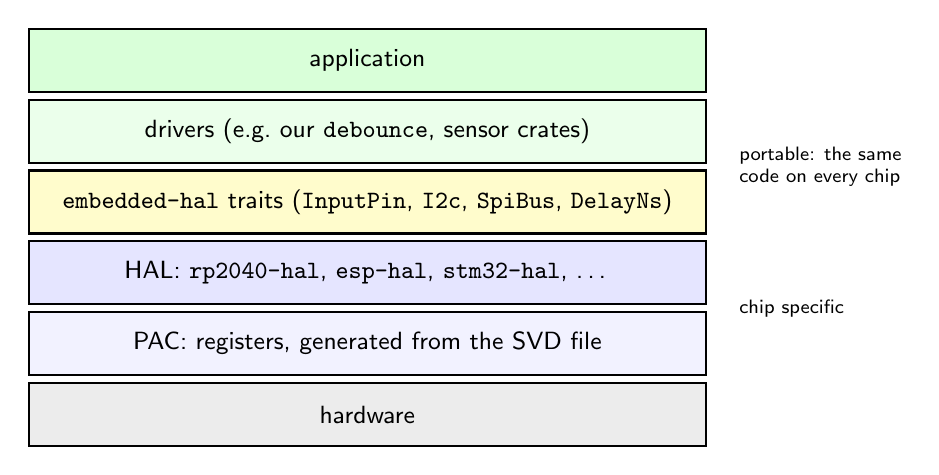
\begin{tikzpicture}[font=\sffamily\small,
	l/.style={draw,thick,minimum width=86mm,minimum height=8mm,align=center}]
	\node[l,fill=green!15] at (0,3.6) {application};
	\node[l,fill=green!8] at (0,2.7) {drivers (e.g.\ our \texttt{debounce}, sensor crates)};
	\node[l,fill=yellow!20] at (0,1.8) {\texttt{embedded-hal} traits (\texttt{InputPin}, \texttt{I2c}, \texttt{SpiBus}, \texttt{DelayNs})};
	\node[l,fill=blue!10] at (0,0.9) {HAL: \texttt{rp2040-hal}, \texttt{esp-hal}, \texttt{stm32-hal}, \ldots};
	\node[l,fill=blue!5] at (0,0) {PAC: registers, generated from the SVD file};
	\node[l,fill=gray!15] at (0,-0.9) {hardware};
	\node[right,font=\sffamily\scriptsize,align=left] at (4.6,2.25) {portable: the same\\code on every chip};
	\node[right,font=\sffamily\scriptsize,align=left] at (4.6,0.45) {chip specific};
\end{tikzpicture}}
\caption{Layers of the embedded Rust ecosystem}
\end{center}
\end{figure}
\os{\newpage}

\item[{\rot\bf A hardware independent driver}]~\\[-3ex]
\begin{lstlisting}[language=Rust]
#![no_std]
use embedded_hal::digital::InputPin;
pub enum Edge { None, Pressed, Released }
pub struct Debouncer { stable: bool, counter: u8, threshold: u8 }  // threshold = samples

impl Debouncer {
    pub fn update(&mut self, raw: bool) -> Edge {
        if raw == self.stable {
            self.counter = 0;
            return Edge::None;
        }
        self.counter += 1;
        if self.counter < self.threshold {
            return Edge::None;
        }
        self.counter = 0;
        self.stable = raw;
        if raw { Edge::Pressed } else { Edge::Released }
    }

    pub fn poll<P: InputPin>(&mut self, pin: &mut P) -> Result<Edge, P::Error> {
        Ok(self.update(pin.is_low()?))   // any pin type that implements InputPin
    }
}
\end{lstlisting}
\os{\newpage}

\item[{\rot\bf Testing embedded code on the PC}]~\\[-3ex]
\begin{lstlisting}[language=Rust]
#[test]
fn bouncing_gives_one_edge() {
    let mut d = Debouncer::new(3);
    // contact bounce: short pulses before the level is stable
    let samples = [true, false, true, false, true, true, true, true, true];
    assert_eq!(run(&mut d, &samples), (1, 0));
}

/// A fake pin for tests: implements the same trait as a real GPIO pin.
struct FakePin(bool);
impl InputPin for FakePin { /* is_high / is_low return self.0 */ }
\end{lstlisting}
\begin{lstlisting}[language={}]
$ cargo test
test tests::bouncing_gives_one_edge ... ok
test tests::clean_press_and_release ... ok
test tests::poll_reads_active_low_pin ... ok
test tests::short_glitch_is_ignored ... ok
test result: ok. 4 passed; 0 failed
\end{lstlisting}
\bi
	\ite the same library runs unchanged on the Pico (\texttt{button\_lib.rs}) -- logic is tested quickly on the PC (or Replit), only the hardware access needs the target
\ei
\os{\newpage}

\item[{\rot\bf Rust tools and practices}]~\\[-3ex]
\bi
	\ite \texttt{rustup target add thumbv6m-none-eabi} / \texttt{riscv32imc-unknown-none-elf}: cross compilation without a separate toolchain
	\ite \texttt{cargo}: build, dependencies (\texttt{Cargo.toml}, \texttt{Cargo.lock} for reproducible builds), tests, documentation
	\ite \texttt{cargo clippy} (lints), \texttt{cargo fmt} (formatting)
	\ite \texttt{probe-rs}: flashing and debugging via SWD/JTAG; \texttt{defmt}: compact logging, formatted on the PC
	\ite errors are values: \texttt{Result<T, E>} and \texttt{Option<T>}, propagated with \texttt{?}; \texttt{unwrap()} only where an error really cannot occur
	\ite \texttt{unsafe} for what the compiler cannot check (registers, assembly, FFI to C) -- keep it small and encapsulated in safe functions
	\ite C and Rust can be mixed: \texttt{extern "C"} in both directions
\ei
\os{\newpage}
\end{description}

%%%%%%%%%%%%%%%%%%%%%%%%%%%%%%%%%%%%%%%%%%%%%%%%%%%%%%%%%%%%%%%%%%%%%%%%%%%
\section{Python and MicroPython}
%%%%%%%%%%%%%%%%%%%%%%%%%%%%%%%%%%%%%%%%%%%%%%%%%%%%%%%%%%%%%%%%%%%%%%%%%%%
\nsl{Python plays two roles in embedded development. On the PC it is the
standard language for tools: test scripts, data analysis, communication with
devices, build automation. On the microcontroller itself, MicroPython (and
its variant CircuitPython) implements Python 3 in about 256\,KB of flash.
The program is interpreted, so it is much slower than C or Rust and the
garbage collector causes pauses. But changes can be tried out at once in the
interactive prompt. This makes MicroPython excellent for prototypes,
teaching and devices where the computing time does not matter.}

\begin{description}
\item[{\rot\bf Python 3 on the PC: working with binary data}]~\\[-3ex]
\begin{lstlisting}[language=Python]
import struct

# 14 bytes from register 0x3B: accel X/Y/Z, temperature, gyro X/Y/Z
raw = bytes.fromhex("0000 0000 4000 f24c 0000 0083 ff7d")

ax, ay, az, temp, gx, gy, gz = struct.unpack(">7h", raw)   # > = big endian, h = int16

accel_g = [v / 16384 for v in (ax, ay, az)]      # +-2 g range: 16384 LSB/g
temp_c = temp / 340 + 36.53                      # formula from the datasheet
print(f"acceleration: {accel_g} g")              # [0.0, 0.0, 1.0] g
print(f"temperature:  {temp_c:.1f} C")           # 26.2 C

packet = struct.pack("BB", 0x6B, 0x00)           # build an I2C write
\end{lstlisting}
\bi
	\ite typical uses: serial port (\texttt{pyserial}), MQTT clients (\texttt{paho-mqtt}), test automation (\texttt{pytest}), plots (\texttt{matplotlib}), Jupyter notebooks for measurements
	\ite always Python 3 -- Python 2 has not been maintained since 2020
\ei
\os{\newpage}

\item[{\rot\bf MicroPython on the Pico}]~\\[-3ex]
\begin{lstlisting}[language=Python]
from machine import ADC, PWM, Pin
import time

pot = ADC(26)
pwm = PWM(Pin(15))
pwm.freq(1000)                  # 1 kHz

while True:
    value = pot.read_u16()      # 0 .. 65535 (12 bit ADC, scaled to 16 bit)
    pwm.duty_u16(value)         # duty cycle 0 .. 100 %
    print(f"ADC {value:5d}  ->  duty {value * 100 // 65535:3d} %")
    time.sleep_ms(200)
\end{lstlisting}
\bi
	\ite the module \texttt{machine} wraps the peripherals: \texttt{Pin}, \texttt{ADC}, \texttt{PWM}, \texttt{I2C}, \texttt{SPI}, \texttt{UART}, \texttt{Timer}
	\ite interrupts: \texttt{button.irq(trigger=Pin.IRQ\_FALLING, handler=f)}; registers: \texttt{machine.mem32[0xd000001c] = 1 << 15}
	\ite runs directly in the browser: new MicroPython Pico project on \url{https://wokwi.com}
	\ite limits: 10 to 100 times slower than C, garbage collection pauses, more RAM -- time-critical parts can be written in C as native modules
\ei
\os{\newpage}
\end{description}

%%%%%%%%%%%%%%%%%%%%%%%%%%%%%%%%%%%%%%%%%%%%%%%%%%%%%%%%%%%%%%%%%%%%%%%%%%%
\section{Debugging}
%%%%%%%%%%%%%%%%%%%%%%%%%%%%%%%%%%%%%%%%%%%%%%%%%%%%%%%%%%%%%%%%%%%%%%%%%%%
\nsl{Debugging embedded systems is harder than debugging PC programs. The
program runs on another device, often without a screen. Timing matters and
changes when you observe it, and the error may lie in the hardware, in the
software or between them. A systematic procedure and the right tools save
a lot of time. This section describes both, with a real example from the
preparation of this lecture.}

\begin{description}
\item[{\rot\bf A systematic approach}]~\\[-3ex]
\bi
	\ite \textbf{reproduce}: find a way to make the error appear reliably -- an error that cannot be reproduced cannot be verified as fixed
	\ite \textbf{observe}: collect facts (output, signals, register values) instead of guessing
	\ite \textbf{hypothesis}: one possible cause that explains all observations
	\ite \textbf{experiment}: a test that confirms or refutes the hypothesis -- change one thing at a time
	\ite \textbf{isolate}: halve the search space (comment out half of the code, \texttt{git bisect} to find the commit that introduced the error)
	\ite \textbf{fix and secure}: correct the cause, not the symptom; add a test that would have found the error
	\ite write down what you have tried -- especially when the error takes days
\ei
\os{\newpage}

\item[{\rot\bf A real case: the flaky button}]~\\[-3ex]
\bi
	\ite symptom: the Rust debouncing example (chapter 6) toggled the LED in some simulation runs and not in others; the C version always worked
	\ite observation 1: the debouncer library passes all unit tests $\Rightarrow$ the logic is probably correct
	\ite observation 2 (GDB): the breakpoint where a new level is accepted is never reached
	\ite observation 3 (diagnostic output with timestamps): dozens of ``pressed''/``released'' events within \textbf{one} millisecond -- the loop runs much faster than once per millisecond
	\ite hypothesis: \texttt{delay.delay\_ms(1)} does not wait 1\,ms
	\ite experiment: measure the delays with the RP2040 hardware timer
	\bi
		\ite \texttt{delay 1 ms: SysTick 4 us, TIMER 1000 us}
		\ite \texttt{delay 500 ms: SysTick 365788 us, TIMER 500001 us}
	\ei
	\ite cause: the SysTick-based delay does not work correctly in the simulator; fix: use the RP2040 timer as delay provider (it implements the same \texttt{DelayNs} trait)
\ei
\os{\newpage}

\item[{\rot\bf Tools without a debugger}]~\\[-3ex]
\bi
	\ite \textbf{output} via UART or USB (\texttt{printf}, \texttt{println!}, logging frameworks)
	\bi
		\ite simple and powerful, but changes the timing: a line at 115200 baud takes milliseconds
		\ite faster alternatives: binary logging (\texttt{defmt}), RTT (output through the debug probe, no UART needed)
	\ei
	\ite \textbf{GPIO toggles} + logic analyzer or oscilloscope: measure timing in microseconds with almost no influence
	\ite \textbf{assertions}: \texttt{assert()} / \texttt{assert!()} check assumptions and stop early instead of failing later
	\ite \textbf{fault handlers}: on a HardFault or panic print the program counter and a backtrace (\texttt{esp-backtrace} in our ESP32 examples)
	\ite \textbf{watchdog} and reset reason: find out that and why the device restarted
\ei
\os{\newpage}

\item[{\rot\bf GDB: the debugger}]~\\[-3ex]
\begin{center}
\resizebox{0.9\textwidth}{!}{%
\begin{tabular}{|l|l|}
\hline
\textbf{command} & \textbf{function} \\
\hline
\texttt{target remote localhost:3333} & connect to the debug server (probe, OpenOCD, probe-rs, Wokwi) \\
\texttt{break func} / \texttt{break file.rs:42} & breakpoint \\
\texttt{continue}, \texttt{next}, \texttt{step}, \texttt{finish} & run, next line, into a function, out of the function \\
\texttt{stepi}, \texttt{display/i \$pc} & one machine instruction, show the next instruction \\
\texttt{backtrace} & call stack \\
\texttt{print var}, \texttt{info registers} & variables and registers \\
\texttt{x/6hu addr} & memory: 6 halfwords, unsigned decimal \\
\texttt{watch var} & watchpoint: stop when the variable is written \\
\hline
\end{tabular}}
\end{center}
\bi
	\ite GDB needs the ELF file with debug information (\texttt{debug = 2} in our \texttt{Cargo.toml})
	\ite graphical front ends: VS Code (Cortex-Debug, probe-rs extension), Eclipse-based IDEs
\ei
\os{\newpage}

\item[{\rot\bf GDB session with the Wokwi simulator}]~\\[-3ex]
\begin{lstlisting}[language={}]
$ wokwi-cli -g 3333 .                       # simulation waits for GDB
$ arm-none-eabi-gdb target/thumbv6m-none-eabi/release/asm_sum
(gdb) target remote localhost:3333
(gdb) break asm_sum
(gdb) continue
Breakpoint 1, 0x100001fe in asm_sum ()
(gdb) info registers r0 r1
r0             0x2003ffd4          537133012      <- address of the array
r1             0x6                 6              <- n
(gdb) x/6hu $r0
0x2003ffd4:     1       2       3       1000    60000   65535
(gdb) stepi 4
(gdb) display/i $pc
1: x/i $pc
=> 0x10000206 <asm_sum+10>:     adds    r2, r2, r3
(gdb) finish
0x10000354 in asm_sum::__cortex_m_rt_main () at src/bin/asm_sum.rs:67
67      let s_asm = unsafe { asm_sum(data.as_ptr(), data.len() as i32) };
\end{lstlisting}
\bi
	\ite in VS Code: ``Wokwi: Start Simulator and Wait for Debugger'', then start a GDB debug session -- breakpoints in the source code
\ei
\os{\newpage}

\item[{\rot\bf Debugging a Linux program without hardware}]~\\
\bi
	\ite on embedded Linux the debugger works on a process, not on the whole chip
	\ite QEMU user mode runs the ARM program on the PC and offers a GDB server (\texttt{-g}); the debugger of the Yocto SDK connects to it (chapter Operating Systems, \texttt{examples/linux})
\ei
\begin{lstlisting}[language={}]
$ qemu-aarch64 -L $SDKTARGETSYSROOT -g 1234 ./sensor_avg &      # waits for GDB
$ $GDB ./sensor_avg                                            # aarch64-poky-linux-gdb
(gdb) set sysroot /path/to/sdk/sysroots/cortexa57-poky-linux
(gdb) target remote :1234
(gdb) break sensor_avg.c:18
(gdb) continue
(gdb) display sum
(gdb) continue
1: sum = 200 '\310'           <- after the first value
(gdb) continue
1: sum = 154 '\232'           <- 200 + 210 = 410 does not fit into uint8_t: 410 - 256
(gdb) continue
1: sum = 88 'X'
\end{lstlisting}
\nsl{With \texttt{-Og} the variable \texttt{sum} lives in a register, so a watchpoint on it fails; \texttt{display} at a breakpoint works.}
\os{\newpage}

\item[{\rot\bf On a real Linux board: gdbserver}]~\\[-3ex]
\bi
	\ite the program runs on the board under \texttt{gdbserver}; GDB runs on the PC with the symbols and the sources
\ei
\begin{lstlisting}[language={}]
board$ gdbserver :1234 ./sensor_avg
pc$    $GDB ./sensor_avg
(gdb)  target remote 192.168.7.2:1234
\end{lstlisting}
\bi
	\ite the board needs \texttt{gdbserver} in the image (Yocto: \texttt{IMAGE\_INSTALL:append = " gdbserver"}; the prebuilt \texttt{core-image-sato-sdk} contains it)
	\ite the binary on the board may be stripped; GDB on the PC uses the unstripped copy and the SDK sysroot for the libraries
	\ite crashes after the fact: enable core dumps on the board, analyse them on the PC with \texttt{\$GDB ./program core}
	\ite kernel problems: messages with \texttt{dmesg}, kernel debugging via QEMU's GDB stub (\texttt{-s -S}) or JTAG
\ei
\os{\newpage}

\item[{\rot\bf Hardware debugging: JTAG and SWD}]~\\[-3ex]
\bi
	\ite on real hardware the debugger talks to the debug unit in the chip through a \textbf{debug probe}
	\ite \textbf{JTAG} (IEEE 1149.1): signals TCK (clock), TMS (mode), TDI (data in), TDO (data out)
	\bi
		\ite originally designed to test soldered boards: \textbf{boundary scan} reads and sets every pin of a chip through a shift register chain -- without the chip's software
		\ite a 16-state machine (TAP controller), driven by TMS, selects instruction and data registers
		\ite several chips can be chained
	\ei
	\ite \textbf{SWD} (serial wire debug, ARM): the same debug functions with only two pins (SWDIO, SWCLK) -- RP2040, STM32 and all Cortex-M
	\ite functions: halt, single step, read and write registers and memory, hardware breakpoints and watchpoints, programming the flash
	\ite probes: Raspberry Pi Debug Probe and other CMSIS-DAP probes, SEGGER J-Link, ST-LINK; the ESP32-C3 has a USB-JTAG unit built in
	\ite software: OpenOCD or \texttt{probe-rs} as GDB server
\ei
\os{\newpage}

\item[{\rot\bf Exercises}]~\\[-3ex]
\bi
	\ite Look at the sections of one of your programs with \texttt{size} or \texttt{llvm-size}. Add a global array \texttt{int a[100] = \{1\};} -- which section grows? And with \texttt{= \{0\}}?
	\ite Write \texttt{asm\_max(const int32\_t *a, int n)} in Thumb assembly (signed maximum) and call it from C or Rust. Test with negative numbers.
	\ite Step through \texttt{asm\_sum} with GDB and watch the flags in \texttt{xpsr} after \texttt{subs}.
	\ite Add a test to the \texttt{debounce} crate: a press that is shorter than the threshold must not produce an edge. Run \texttt{cargo test} on Replit.
	\ite Port \texttt{adc\_pwm.py} to C and to Rust (chapter 6 contains all parts). Compare code size and effort.
	\ite In C: why is \texttt{(uint8\_t)200 + (uint8\_t)100 > 255} true? Check it on the PC.
	\ite Linux: debug \texttt{examples/linux/sensor\_avg.c} with QEMU user mode and the GDB of the Yocto SDK. Fix the bug and check the result on the emulated board.
\ei
\end{description}
